\documentclass[UTF8]{ctexart}
\usepackage{graphicx}
\usepackage{amsmath}
\usepackage{bibentry,natbib}
\usepackage{fancyhdr}

\title{Machine Learning Note}
\author{BrightHush}
\date{\today}

\begin{document}
\maketitle
\tableofcontents

\pagestyle{fancy}
\cfoot{\thepage}

\newcommand{\figref}[1]{\figurename~\ref{#1}}

\section{Restricted Boltzmann Machine}
RBM 是 Boltzmann Machine 的一种,在 RBM 中,同一层中的单元不存在连接。

\subsection{Architecture of RBM}
RBM 其实就是一个二分图,只有两层,一个可见层和一个隐藏层,其结构如图\ref{Fig:RBM}。
\begin{figure}[h!] 
    \centering     
    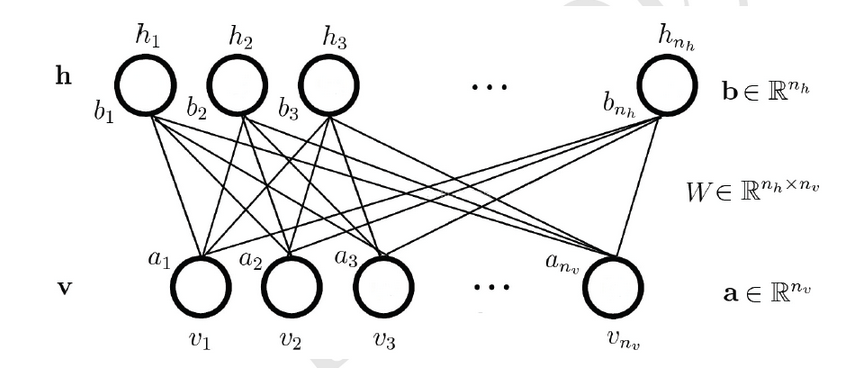
\includegraphics[width=1.0\textwidth]{rbm}   
    \caption{\label{Fig:RBM}RBM Architecture} 
\end{figure}
\par
RBM的变量表示方法在\ref{Fig:RBM}已经描绘出来,可见层是用\textbf{v}表示,隐层使用\textbf{h}表示,
其中需要注意的是权值矩阵$W \in R^{n_h \times n_v} $,也就是说$ W_{ij} $表示隐层第i个单元与可见层
第j个单元的连接权重。模型的参数为$ \theta = (W, a, b) $,其中$ (a, b)$分别表示可见层和隐藏层的偏置。
\par
通常来说,我们讨论的RBM的每个神经元的取值为二元的,也就是取值为0或者1。

\subsection{Energy Function and Probability Distribution}
RBM是一个基于能量的物理模型,通过定义能量函数,我们就可以表示该系统的联合概率了。RBM中,对于给定的状态
(\textbf{v}, \textbf{h}),其能量函数表示为(\ref{EnergyFunction})。
\begin{align}
\label{EnergyFunction}
E_{\theta}(\textbf{v}, \textbf{h}) &= 
 -\sum_{i=1}^{n_v}a_i v_i - \sum_{j=1}^{n_h}b_j h_j 
 - \sum_{i=1}^{n_v} \sum_{j=1}^{n_h} h_j W_{ji} v_i
\end{align}
表示成矩阵向量形式为(\ref{VectorizedEnergyFunction})。
\begin{align}
\label{VectorizedEnergyFunction}
E_{\theta}(\textbf{v}, \textbf{h}) &= 
 -a^T v - b^T h - h^T W v
\end{align}
\par
在能量函数如(\ref{EnergyFunction})给定的情况下,定义状态(\textbf{v}, \textbf{h})的联合概率表示为
(\ref{JointDistribution})。
\begin{align}
\label{JointDistribution}
P_{\theta}(\textbf{v}, \textbf{h}) &= 
  \frac{e^{-E_{\theta}(v, h)}}{Z_{\theta}}
\\
in \ which : Z_{\theta} &= \sum_{v}\sum_{h} e^{-E_{\theta}(v, h)}
\end{align}
\par
有了联合概率分布,我们可以得到边缘概率分布$P_{\theta}(v), P_{\theta}(h)$,也就是我们常说的
似然函数(likelihood function),其表示为\ref{MarginDistrition}
\begin{align}
\label{MarginDistrition}
P_{\theta}(v) &= \sum_{h}P_{\theta}(v, h) \\
&= \frac{1}{Z_{\theta}} \sum_{h}e^{-E_{\theta}(v, h)}
\\
P_{\theta}(h) &= \sum_{v}P_{\theta}(v, h) \\
&= \frac{1}{Z_{\theta}} \sum_{v}e^{-E_{\theta}(v, h)}
\end{align}

\par 通过定义能量函数以及使用能量函数表示的联合概率分布,以及RBM中的条件独立关系,可以推导出下面的
两个类似普通神经网络中的 forward propagation 的计算公式(\ref{ConditionalProbability})。
\begin{align}
\label{ConditionalProbability}
P(h_k=1|v) &= sigmoid(b_k + \sum_{i=1}^{n_v} W_{ki}v_i)
\\
p(v_k=1|h) &= sigmoid(a_k + \sum_{j=1}^{n_h} h_j W_{jk})
\end{align}

由于已知可见层的情况下,隐层各单元之间条件独立;已知隐层的情况下,各可见层单元条件独立。于是可以得到
在已知某一层的情况下,另一层状态的条件概率表达式。
\begin{align}
p(h|v) &= \Pi_{j=1}^{n_h} p(h_j|v)
\\
p(v|h) &= \Pi_{i=1}^{n_v} p(v_i|h)
\end{align}

\subsection{Likelihood Function}
通常来说一个模型需要优化的目标要么是最小化损失函数,要么是最大化似然函数,目的只有一个,那就是要最好的
拟合当前的训练样本集合。在RBM中,我们需要最大化的是模型计算的样本似然。
\par
假设我们的样本集合为
\[ S = {v^1, v^2, ..., v^n} \]
其中$v^i$表示第i个样本,显然我们认为这些样本是独立同分布的,那么我们训练RBM的目标就是最大化下面的似然
函数(\ref{RBMlikelihood})
\begin{align}
\label{RBMlikelihood}
L_{\theta, S} = \Pi_{v^i \in S} P(v^i)
\end{align}
将上述似然转化成为log似然,于是取对数便得到
\begin{align}
ln(L_{\theta, S}) = \sum_{v^i \in S} ln(P(v^i))
\end{align}

\subsection{Gradient Computation}
最大化上述的log似然,我们通常采用梯度上升法,表示为
\begin{align}
\theta := \theta + \eta \frac{\partial ln(L_S)}{\partial \theta}
\end{align}
不管是 Batch Gradient 还是 Statistic Gradient 算法,我们都需要分别计算每一个样本下的梯度变化,因此
我们需要首先推导单个样本下的梯度计算公式,对于单个样本,我们计算
\begin{align}
ln(L_S) &= ln(P(v))
\\
&= ln(\sum_h p(v, h)) 
\\
&= ln(\sum_h \frac{e^{-E(v, h)}}{Z})
\\
&= ln(\sum_h e^{-E(v, h)}) - ln(\sum_v \sum_h e^{-E(v, h)})
\end{align}
上式对参数求导可以表示为
\begin{align}
\label{thetaGradient}
\frac{\partial ln(P(v))}{\partial \theta} 
&= -\sum_h P(h|v) \frac{\partial E(v, h)}{\partial \theta} + 
\sum_{v,h} P(v, h) \frac{\partial E(v, h)}{\partial \theta}
\end{align}
(\ref{thetaGradient})前一项可以看成为对应条件概率的期望,第二项看成是对于联合概率的期望。
(\ref{thetaGradient})可以进一步表示为
\begin{align}
\label{ThetaGradient}
\frac{\partial ln(P(v))}{\partial \theta} 
&= -\sum_h P(h|v) \frac{\partial E(v, h)}{\partial \theta} + 
\sum_v P(v) \sum_h P(h|v) \frac{\partial E(v, h)}{\partial \theta}
\end{align}
于是我们只需要计算$\theta$中各个参数对应$\sum_h P(h|v) \frac{\partial E(v, h)}{\partial \theta}$的
情况,下面进行推导。
对$W_ij$进行求导,
\begin{align}
\label{wGradient}
\sum_h P(h|v) \frac{\partial E(v, h)}{\partial W_{ij}} &=
- \sum_h P(h|v)h_i v_j \\
&= - v_j \sum_h P(h_i|v)P(h_{-i}|v) h_i \\
&= - v_j \sum_{h_i} \sum_{h_{-i}} P(h_i|v)h_i P(h_{-i}|v) \\
&= - v_j \sum_{h_i} P(h_i|v)h_i \sum_{h_{-i}} P(h_{-i}|v) \\
&= - v_j \sum_{h_i} P(h_i|v)h_i \\
&= - v_j (P(0|v)0 + P(1|v)1) \\
&= - v_j P(h_i=1|v)
\end{align}
对$a_i$进行求导,
\begin{align}
\sum_h P(h|v)\frac{\partial E(v, h)}{\partial a_i} &=
- \sum_h P(h|v) v_i \\
&= - v_i
\end{align}
对$b_i$进行求导,
\begin{align}
\sum_h P(h|v)\frac{\partial E(v, h)}{\partial b_i} &=
- \sum_h P(h|v) h_i \\
&= - P(h_i=1|v)
\end{align}
将上述式子分别代入到 \ref{ThetaGradient} 中,我们可以得到各项梯度计算函数为
\begin{align}
\label{Wgradient}
\frac{\partial ln(P(v))}{\partial W_{ij}} 
&= v_jP(h_i=1|v) - \sum_v P(v) P(h_i=1|v)v_j
\end{align}

\begin{align}
\label{agradient}
\frac{\partial ln(P(v))}{\partial a_i} 
&= v_i - \sum_v P(v) v_i
\end{align}

\begin{align}
\label{bgradient}
\frac{\partial ln(P(v))}{\partial b_i} 
&= P(h_i=1|v) - \sum_v P(v) P(h_i=1|v)
\end{align}
\par上述三个公式中,都需要计算$\sum_v$,这个复杂度是$O(2^{n_v})$的。对于这种求期望的形式,
我们通常可以使用采样的方法进行计算,获得样本之后直接计算$\sum_v$即可。如果我们使用Gibbs
采样方法,需要足够次数的状态转移才能保证采样到的样本符合目标分布,然而采集大量的样本则加重了
RBM训练的复杂度,所以在求解RBM参数的时候,通常采用的 Contrastive Divergence 算法来降低
RBM参数训练的复杂度。

\subsection{Contrastive Divergence Algorithm}
在式子(\ref{Wgradient}, \ref{agradient}, \ref{bgradient})中的$\sum_v$的项如果使用
MCMC算法,需要经过较多的步数才能收敛到目标分布。在RBM模型中,我们的目的是要你和训练样本的分布,那么
如果让MCMC从训练样本分布出发,是否会更快的收敛到目标分布呢?基于这个想法,2002年Hinton提出了 Contrastive
Divergence 算法。
在CD-k算法中,依次按照下面的两个步骤进行采样:
\begin{itemize}
\item[•] 通过$P(h^t|v^{t-1})$采样得到$h^t$
\item[•] 通过$P(v^t|h^t)$采样得到$v^t$
\end{itemize}
然后使用$P(v^k|h^k)$代替式子(\ref{Wgradient}, \ref{agradient}, \ref{bgradient})中的$\sum_v$
对应的期望项,其实相当于说我们使用第k次采样得到的样本来近似期望。
\begin{align}
\frac{\partial ln(P(v))}{\partial W_{ij}} 
&= v_j^0 P(h_i=1|v^0) - P(h_i=1|v^k)v_j^k
\\
\frac{\partial ln(P(v))}{\partial a_i} 
&= v_i^0 - v_i^k
\\
\frac{\partial ln(P(v))}{\partial b_i} 
&= P(h_i=1|v^0) - P(h_i=1|v^k)
\end{align}
在实际应用中k取1的时候,就能达到非常好的效果了。通过CD-k算法,现在梯度是可计算的了。

\subsection{Evaluate RBM}
对于已经学习得到或者正在学习的RBM,我们应该如何评价RBM呢?如果我们使用$ln(L_S)$的话,
分母中存在$Z$难以计算。于是我们可以考虑\textbf{重构误差},也就是说以训练样本作为初始
状态,经过一次RBM定义的分布进行一次Gibbs采样得到的$v^{'}$与原始$v$的差异,这个差异
可以定义为1范数或者2范数。显然,重构误差能在很大程度上描述RBM对训练数据拟合的似然情况。


\section{References}
\begin{itemize}
\item[1] Convolutional Neural Networks, \\
\url{http://andrew.gibiansky.com/blog/machine-learning/convolutional-neural-networks/} .
\item[2] 数据挖掘系列(10)卷积神经网络算法的一个实现, \\
\url{http://www.cnblogs.com/fengfenggirl/p/cnn\_ implement.html}.
\item[3] 受限波兹曼机(RBM)学习笔记, \\
\url{http://blog.csdn.net/itplus/article/details/19168937}
\end{itemize}

\end{document}
